\documentclass[11pt]{article}
\usepackage[utf8]{inputenc}
\usepackage[T1]{fontenc}
\usepackage{graphicx}
\usepackage[export]{adjustbox}
\graphicspath{ {./images/} }

\begin{document}
\section*{Reading}
Illiquidity, Accounting Conservatism, IRR, and the J-Curve

As discussed in previous sections, the illiquidity of some alternative investments means that interim IRRs are often based on estimated values rather than market values. These estimated values are usually based on accounting principles that reflect the convention of conservativism. The accounting convention of conservatism holds that it is prudent to recognize potential expenses and liabilities as soon as possible but not to similarly anticipate potential revenues or gains, often resulting in an understatement of income and assets in the short run.

\section*{Accounting Conservatism and Early Fund Losses}
Consider the case of a private equity fund. In the early years of the fund, the fund's management team incurs expenses while selecting investments and otherwise managing the fund. These expenditures are made to build the fund's long-run value. In an economic sense, these expenditures, if prudently made, are likely building value, not depleting value. Nevertheless, there is substantial risk that these expenditures will not create value in the long run. Therefore, accounting conservatism dictates that the expenditures should be expensed immediately rather than capitalized as an asset. The early losses due to managerial and acquisition expenses tend to generate negative interim IRRs in the early years of funds such as private equity funds.

\section*{Accounting Conservatism and Deferred Recognition of Gains}
Another implication of accounting conservatism is to accelerate recognition of losses on investments that are likely to fail and to hold off on fully recognizing potential profits on investments that are progressing nicely. Private equity funds may be likened to gardeners who sow seeds in the knowledge that most will soon fail but those that thrive will eventually generate profits many times their cost. Consider a private equity fund experiencing a normal rate of failure in the early years. Although a few ventures thrive and might reasonably be viewed as gaining in value, the prompt recognition of potential losses will tend to generate early losses and deferred net profits. The result is that interim IRRs of successful funds may not be positive for five or more years.

Financial Accounting Standard (FAS) 157, which was introduced in 2006, seeks to require asset managers to regularly value their investments at fair value, even when the valuation is not immediately observable from market prices. Rather than holding the investment at cost until an impairment or later round of funding forces a change in valuation, the standard seeks more regular changes in value based on both changes in the fortunes of the company as well as valuations of comparable firms. Private equity firms that follow this fair value accounting will likely report company valuations that more accurately predict exit valuations, and have changes in fund NAVs that have higher volatility and higher correlation to liquid financial markets.

\section*{The J-Curve}
The J-curve is a diagram popular in the analysis of private equity that plots IRR on the vertical axis and time since inception on the horizontal axis, generating the fund performance curve often likened in shape to a hockey stick and depicted in the next exhibit, J-Curve of Interim IRRs.

The J-Curve is caused by a combination of early expense recognition, early loss recognition, and deferred gain recognition. The J-Curve therefore depicts an apparent decline in value during the early years of existence, the so-called valley of tears, before beginning to show the hoped-for positive returns in the later years of the fund's life. Beyond five years, the interim IRRs will give a reasonable indication of the final IRR at the fund's maturity. Although the J-Curve of interim IRRs is usually discussed in the context of funds, the J-Curve can also be applied to individual ventures. Many speculative ventures possess the inherent likelihood of shortterm expenses and long-term profits that generate the familiar J-Curve at the venture or company level. After all, it is the aggregation of the outcomes of the individual ventures that forms the fund-level outcome.

\begin{center}
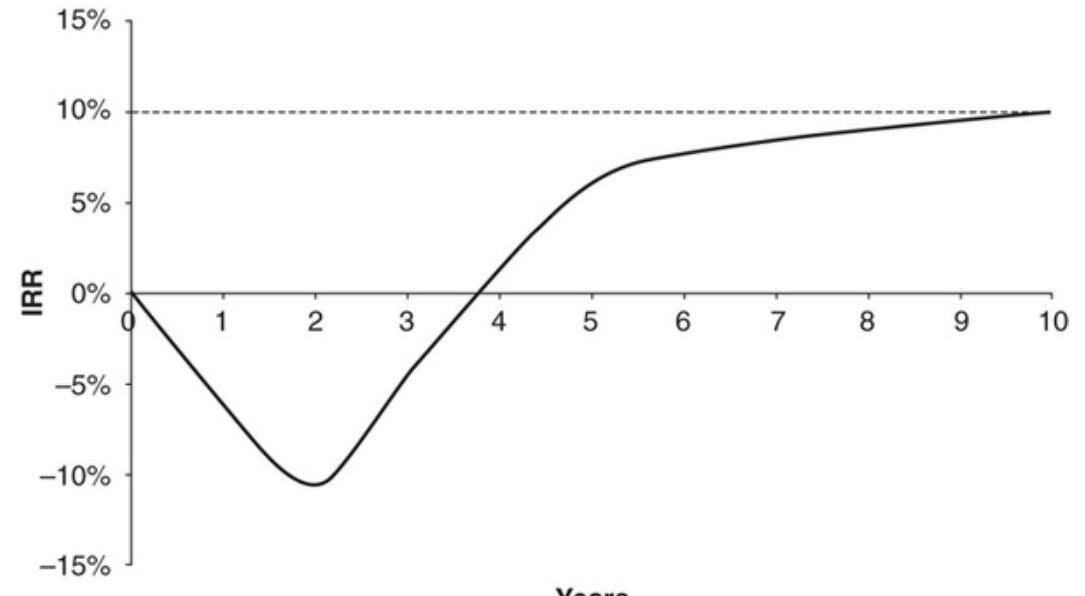
\includegraphics[max width=\textwidth]{2024_04_10_3693761da65f19bde100g-2}
\end{center}

J-Curve of Interim IRRs


\end{document}